\chapter{Проведение моделирования при различных значениях силы связи}
\label{ch:chap8}

\section{Визуализация}

\begin{figure}[h]
	\center{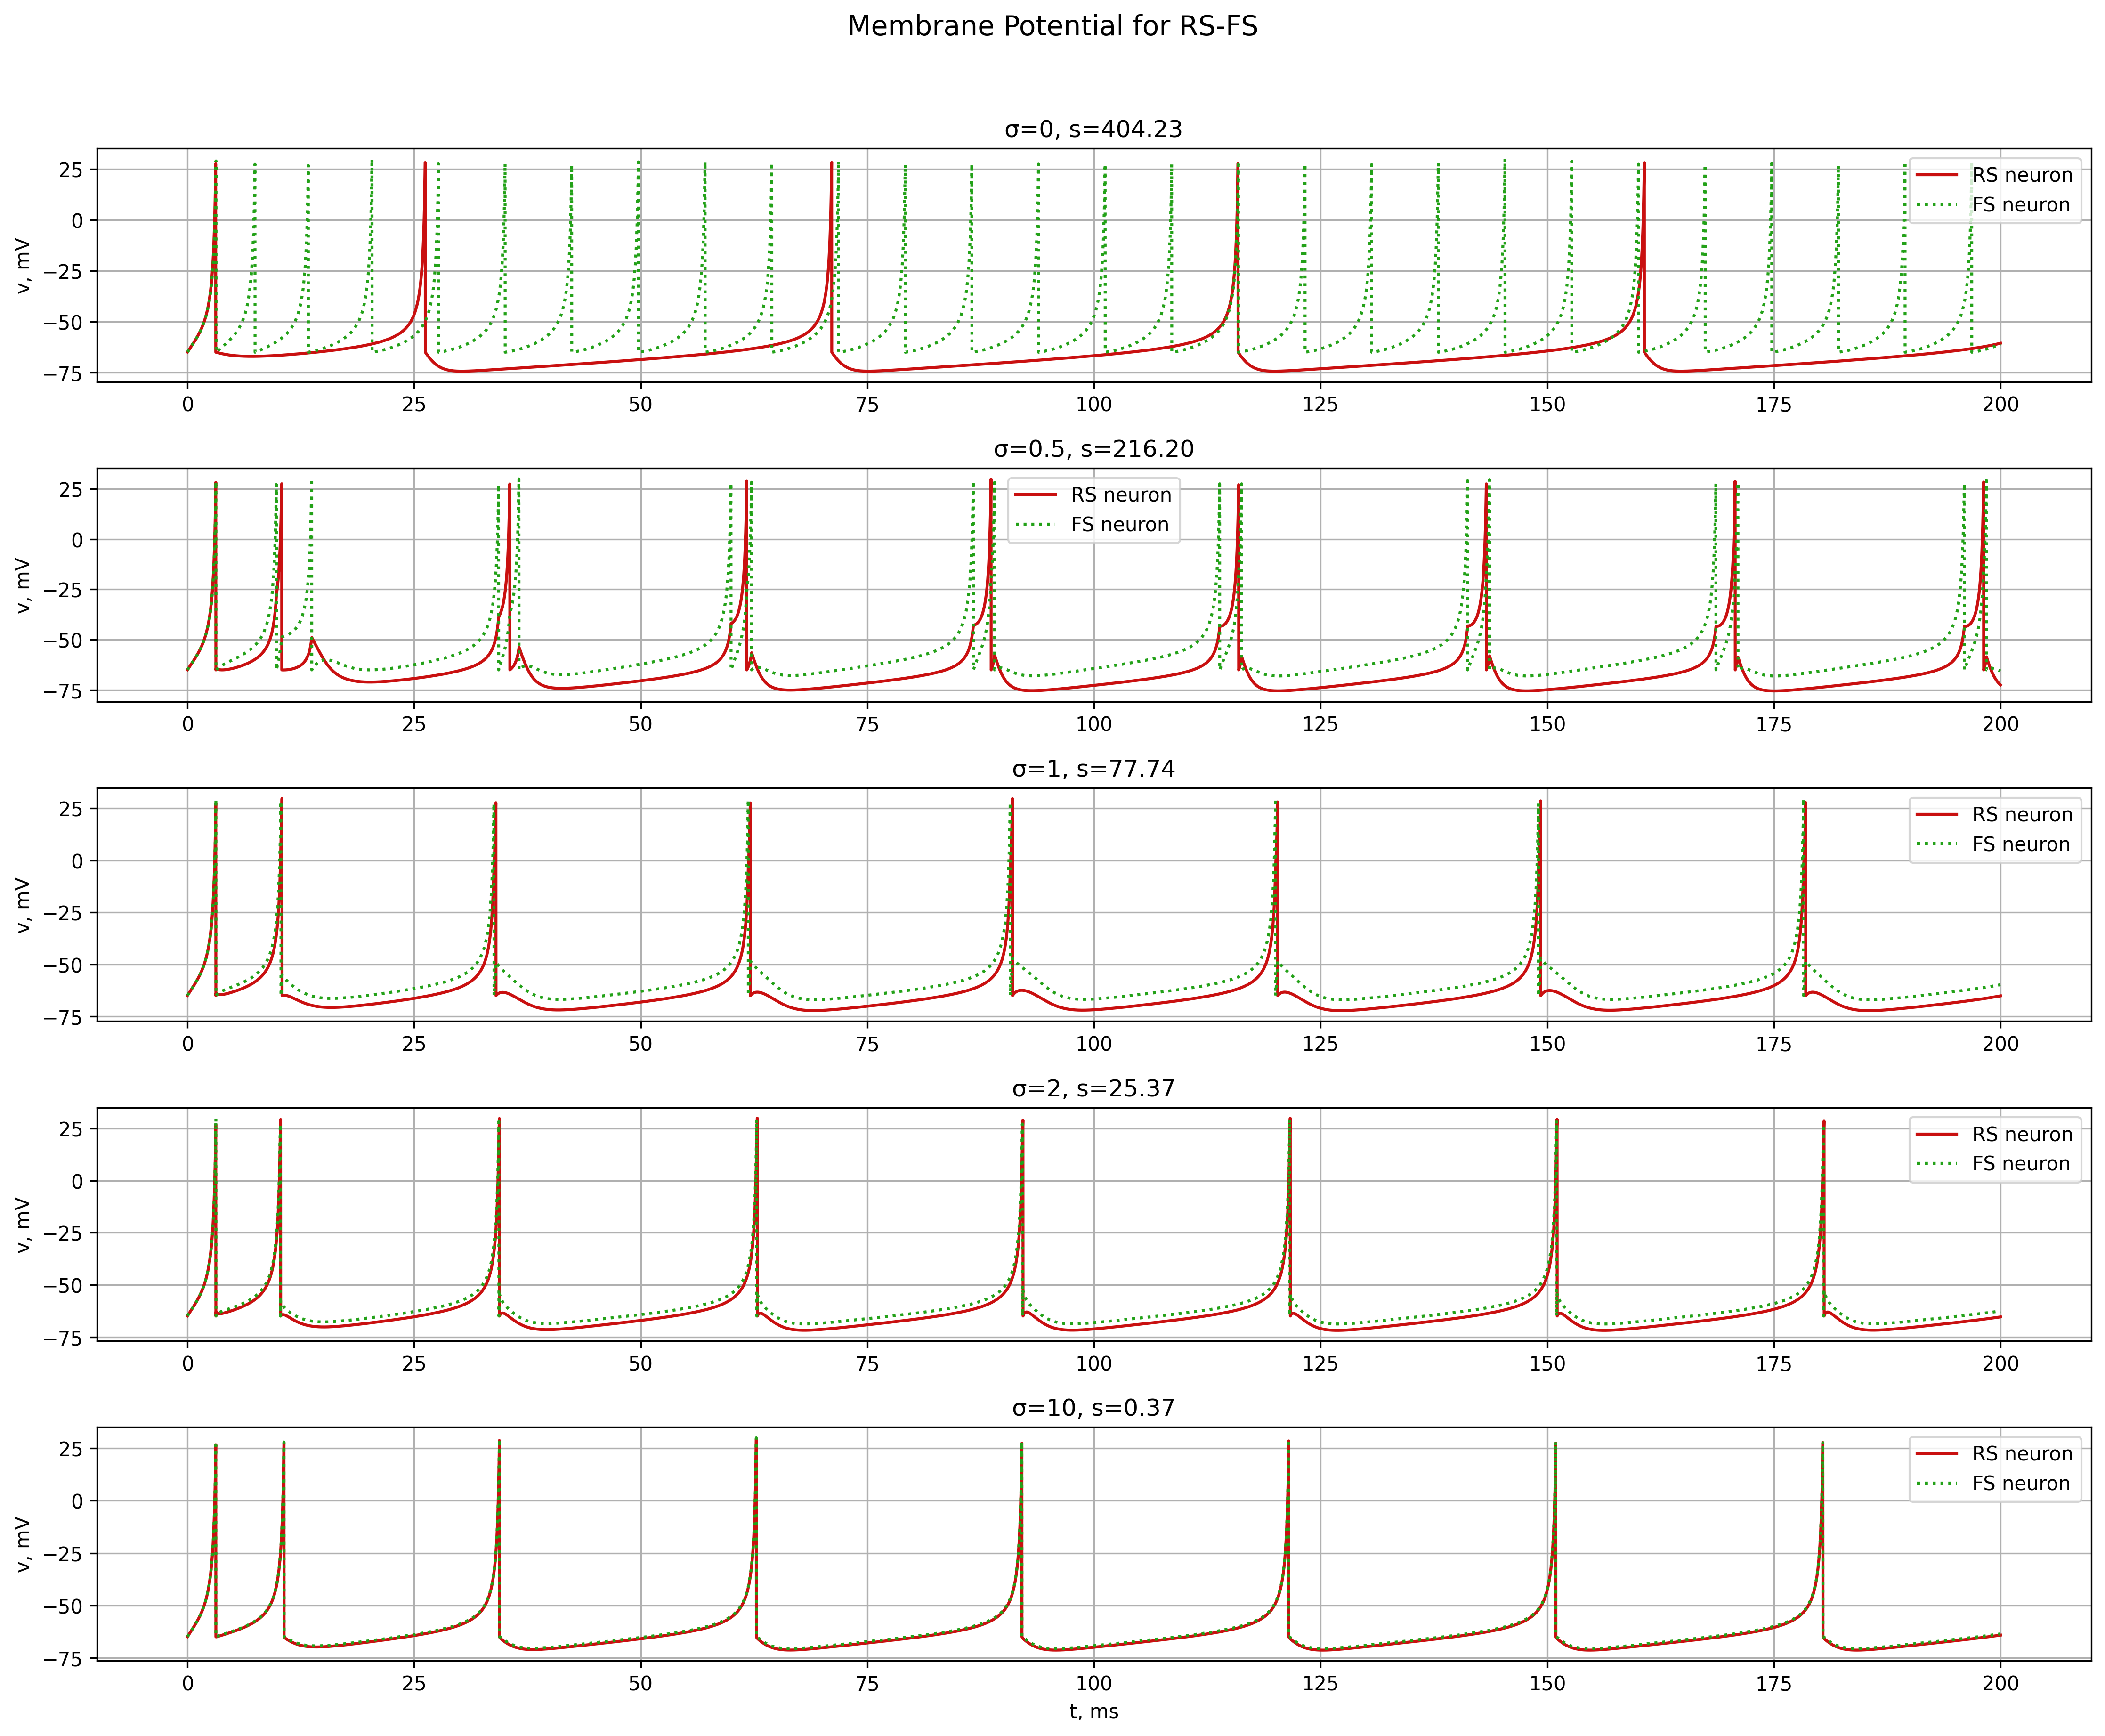
\includegraphics[width=1\linewidth]{pic/v_rsfs.png}}
	\caption{Графики мембранного потенциала $v_i(t)$ нейронов сети для различных значений силы связи.}
	\label{v_rsfs}
\end{figure}

\begin{figure}[h]
	\center{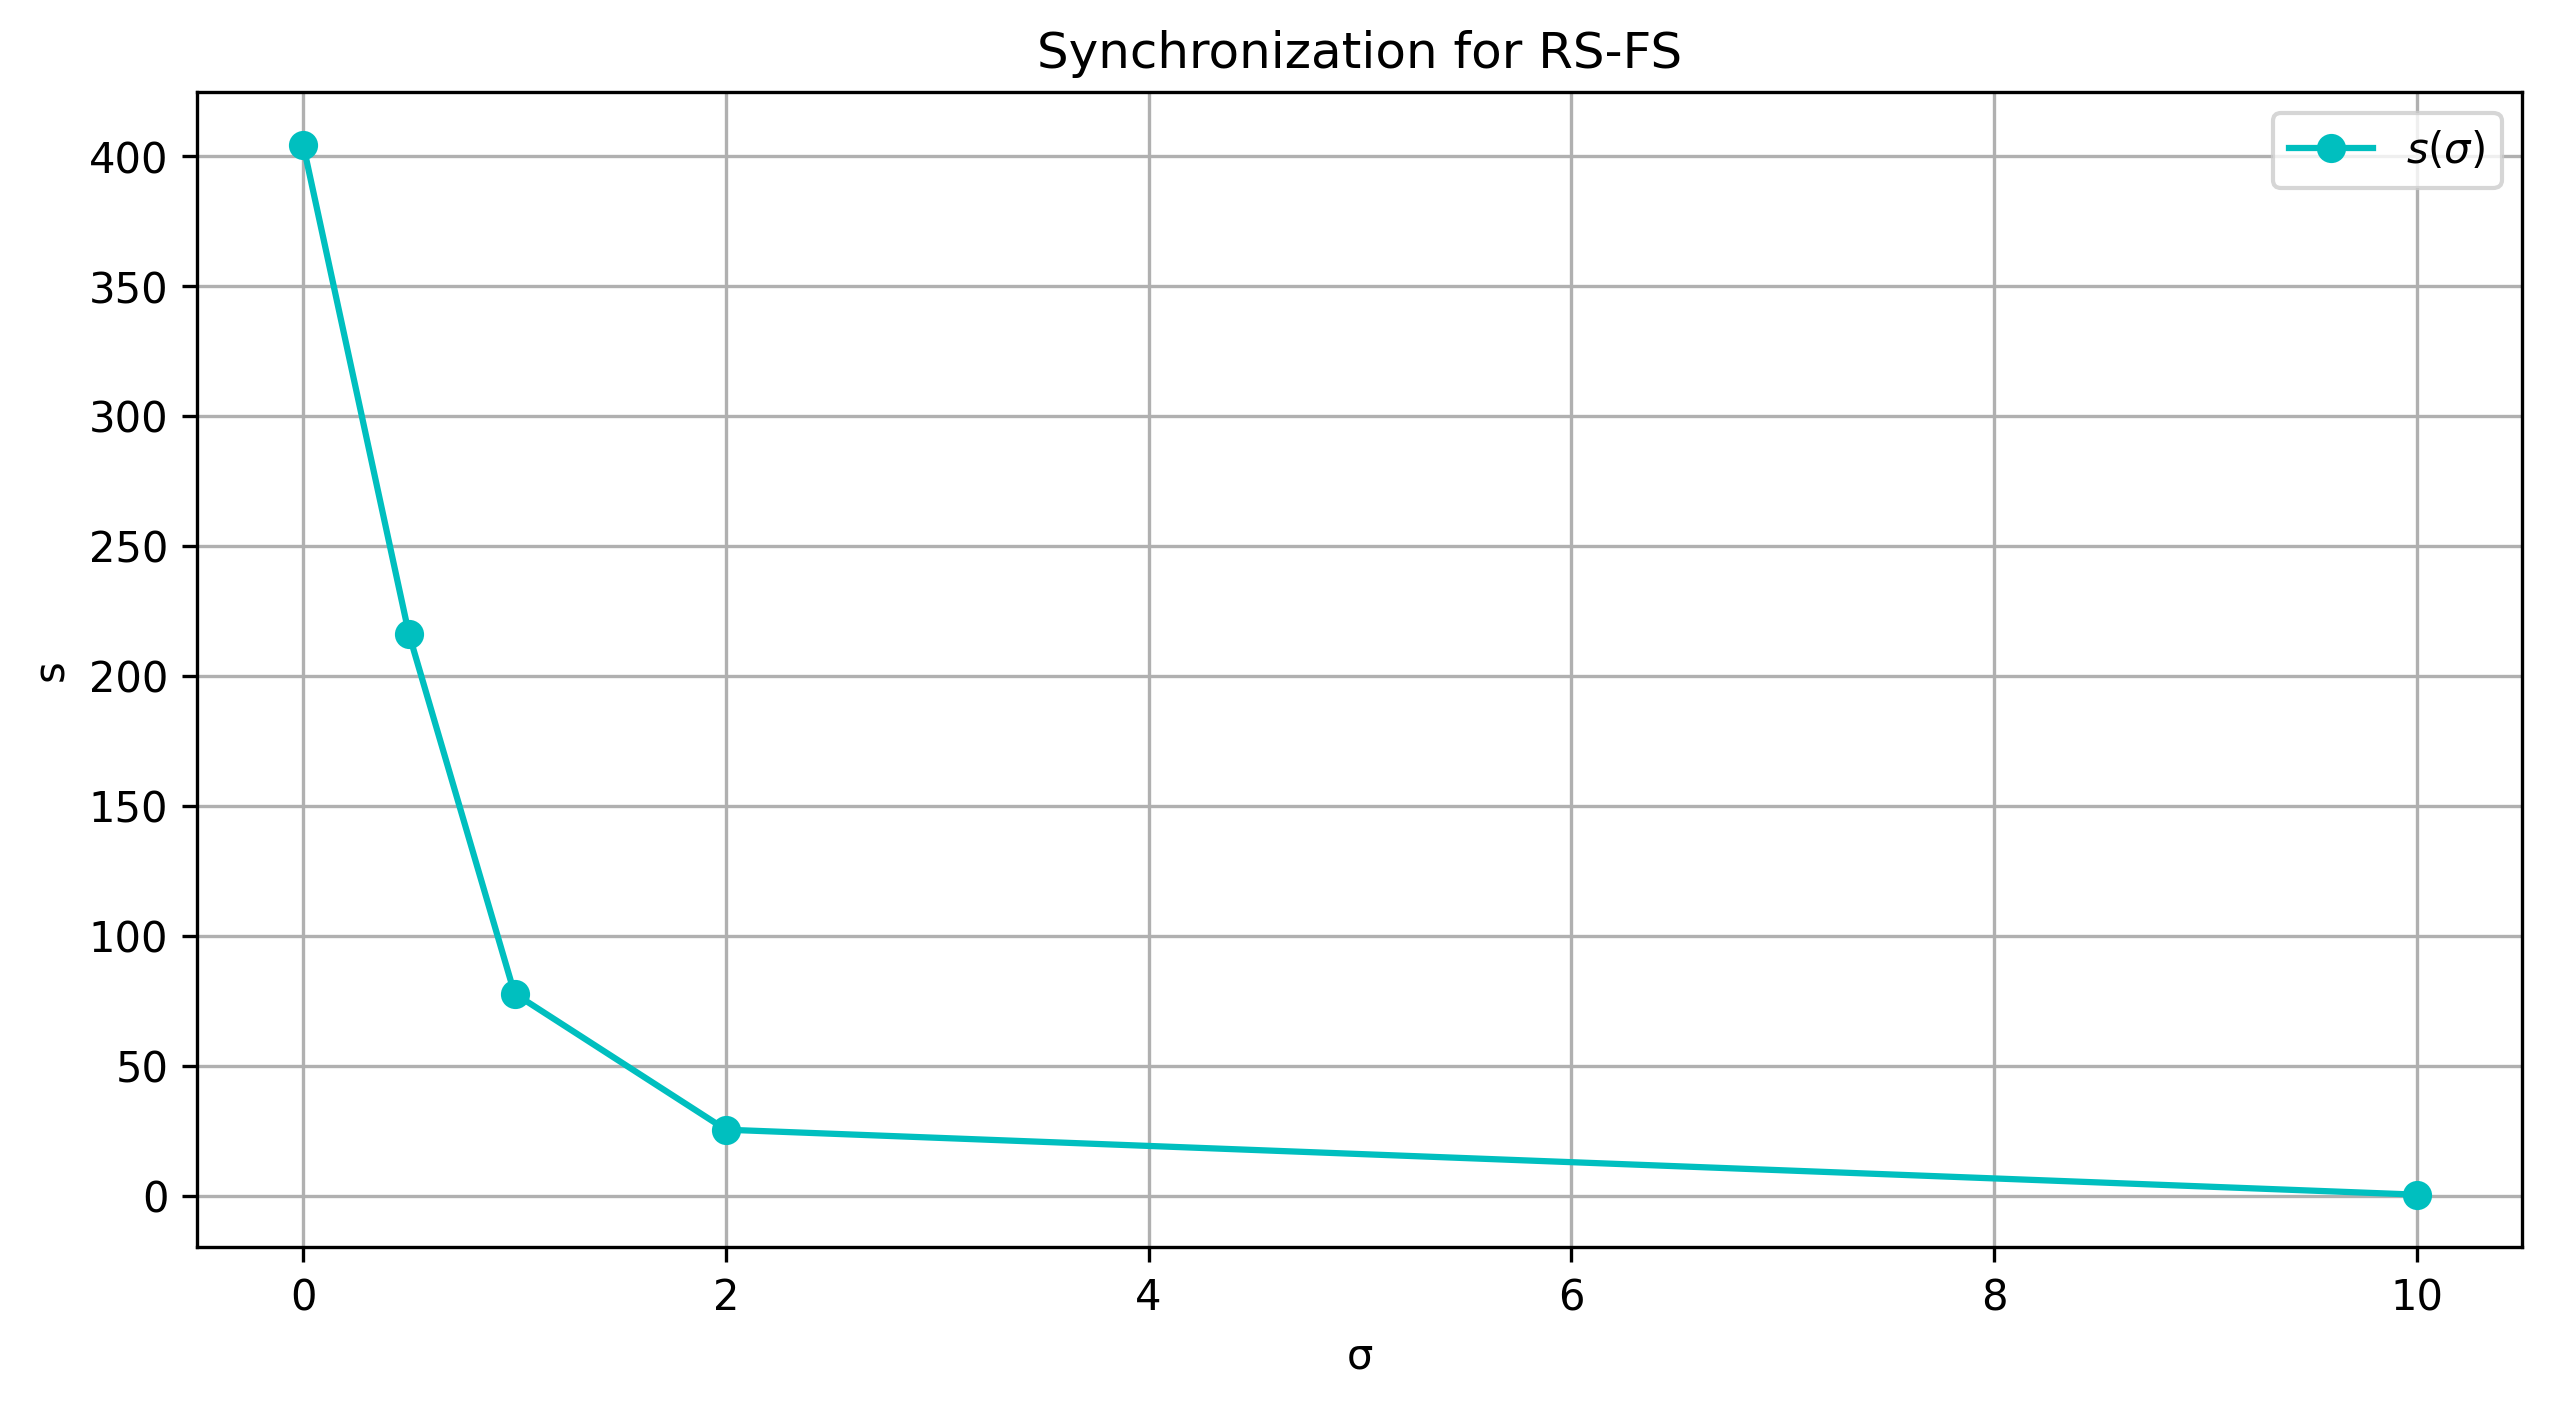
\includegraphics[width=1\linewidth]{pic/sync.png}}
	\caption{График синхронизации $s(\sigma)$ нейронов сети для различных значений силы связи.}
	\label{sync}
\end{figure}

\section{Анализ результатов}
Заметим, что при увеличении значения силы связи возрастает и уровень синхронизации нейронов сети (рисунок \ref{sync}). Кроме того, с увеличением силы связи динамика мембранных потенциалов обоих нейронов меняется, для RS-нейрона характерно повышение частоты спаек, для FS-нейрона -- падение частоты (рисунок \ref{v_rsfs}). В начале временного интервала заметно повышение частоты спаек с последующим увеличением временного интервала между спайками.


\section{Листинг кода}

\inputminted[
breakanywhere=true, 
breaklines=true,
breaksymbolleft=\small\carriagereturn, 
frame=lines,
linenos,
fontsize=\footnotesize,
baselinestretch=0.8
]{python}{big_file2.py}
\captiontextt{Листинг 2 --- Исходный код программы для моделирования динамики сети нейронов.}

\endinput